\section{Modelagem Física}

A estrutura mecânica da bancada — mesa de suporte e células de carga — já era utilizada pela equipe Albatroz Aerodesign em ensaios anteriores. O escopo deste trabalho não abrange a construção dessa estrutura, mas sim sua instrumentação e
integração a um sistema unificado de aquisição, processamento e supervisão. Parte-se, portanto, da bancada existente (\autoref{fig:bancada_fisica}), formalizando-a por meio do acoplamento das placas de medição, do gabinete de instrumentação e da rede de comunicação descritos nesta seção.

\begin{figure}[H]
    \centering
    \caption{Estrutura mecânica da bancada utilizada pela equipe (espaço reservado)}
    \label{fig:bancada_fisica}
    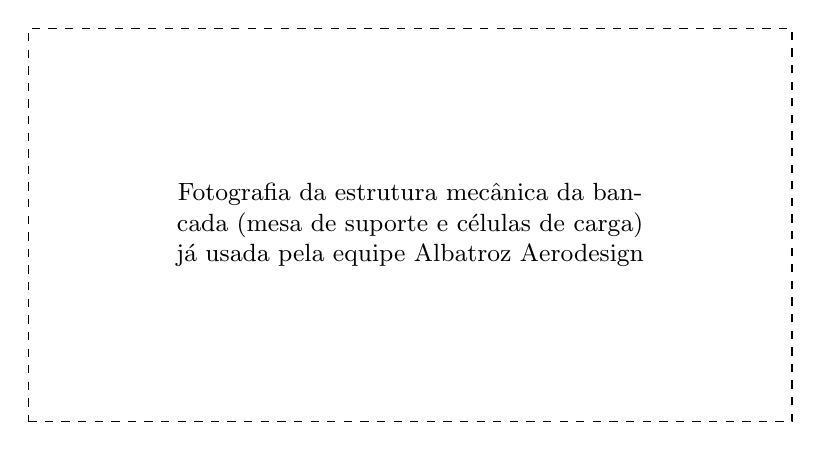
\begin{tikzpicture}
        \node[draw, dashed, align=center, minimum width=0.8\textwidth,
              minimum height=5cm, text width=0.7\textwidth, font=\small]
              {Fotografia da estrutura mecânica da bancada (mesa de suporte
               e células de carga) já usada pela equipe Albatroz Aerodesign};
    \end{tikzpicture}

    Fonte: Autor (2026)
\end{figure}

\subsection{Montagem Final do Conjunto (placeholder)}
\label{sec:resultado_montagem_final}

As figuras a seguir registram o sistema já integrado: o conjunto
motopropulsor montado na bancada, a fiação interna da caixa de
instrumentação após a integração das placas, e o sistema completo em
operação durante um ensaio.

\begin{figure}[H]
    \centering
    \caption{Conjunto motopropulsor (motor e hélice) montado na bancada (espaço reservado)}
    \label{fig:resultado_motor_helice_montado}
    \begin{tikzpicture}
        \node[draw, dashed, align=center, minimum width=0.75\textwidth,
              minimum height=5cm, text width=0.65\textwidth, font=\small]
              {Fotografia do motor com a hélice acoplada, fixado na
               bancada, pronto para ensaio};
    \end{tikzpicture}

    Fonte: Autor (2026)
\end{figure}

\begin{figure}[H]
    \centering
    \caption{Conexões internas da placa após a integração final (espaço reservado)}
    \label{fig:resultado_conexoes_internas}
    \begin{tikzpicture}
        \node[draw, dashed, align=center, minimum width=0.85\textwidth,
              minimum height=6cm, text width=0.75\textwidth, font=\small]
              {Fotografia em detalhe da fiação e dos conectores internos da
               placa/caixa de instrumentação, já integrados};
    \end{tikzpicture}

    Fonte: Autor (2026)
\end{figure}

\begin{figure}[H]
    \centering
    \caption{Bancada completa montada, em operação durante um ensaio (espaço reservado)}
    \label{fig:resultado_bancada_operacao}
    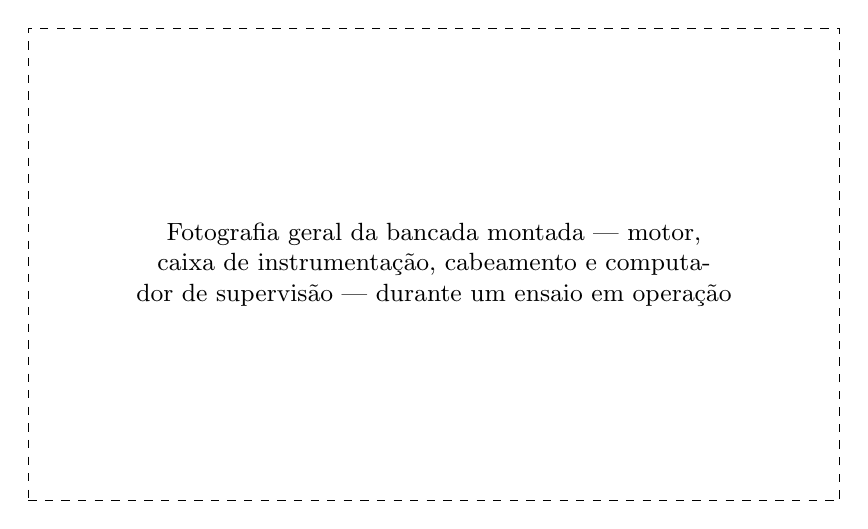
\begin{tikzpicture}
        \node[draw, dashed, align=center, minimum width=0.85\textwidth,
              minimum height=6cm, text width=0.75\textwidth, font=\small]
              {Fotografia geral da bancada montada --- motor, caixa de
               instrumentação, cabeamento e computador de supervisão ---
               durante um ensaio em operação};
    \end{tikzpicture}

    Fonte: Autor (2026)
\end{figure}
